\documentclass[parskip]{scrartcl}
\usepackage[margin=15mm]{geometry}
\usepackage{tikz}
\usepackage{pifont} 
\usepackage{anttor}
\usepackage[utf8]{inputenc}

\graphicspath{ {images/} }

\begin{document}
\pgfmathsetmacro{\cardwidth}{5}
\pgfmathsetmacro{\cardheight}{8}
\pgfmathsetmacro{\stripwidth}{0.6}
\pgfmathsetmacro{\strippadding}{0.1}
\pgfmathsetmacro{\textpadding}{0.1}
\pgfmathsetmacro{\ruleheight}{0.15}

% original card from stack exchange 
%
%\begin{tikzpicture}
%\draw[rounded corners=0.2cm] (0,0) rectangle (\cardwidth,\cardheight);
%\fill[lime,rounded corners=0.1cm] (\strippadding,\strippadding) rectangle (\strippadding+\stripwidth,\cardheight-\strippadding) node[rotate=90,above %left,black,font=\large] {Wizard Spell2 \rotatebox[origin=c]{-90}{\ding{52}}};
%\node[text width=(\cardwidth-\strippadding-\stripwidth-2*\textpadding-0.3)*1cm,below right] at (\strippadding+\stripwidth+\textpadding,\cardheight-\textpadding%) {
%    {\Large KEEPER}\        \vspace{0.15cm}
%    {\scriptsize Lorem ipsum dolor sit amet, consectetur adipisicing elit, sed do eiusmod tempor incididunt ut labore et dolore magna aliqua.\\}%<------modified here
%    \vspace{0.25cm}
%   {{\large {Inter Arma going into two lines\hfill} }} \\[-9pt]% <------modified here
%  \vrule width \textwidth height 3pt \\[-3pt] % <------modified here
%         \tikz{\fill (0,0) rectangle (\cardwidth-\strippadding-\stripwidth-2*\textpadding-0.3,\ruleheight);}\            \vspace{0.2cm}
%        {\scriptsize Lorem ipsum dolor sit amet, consectetur adipisicing elit.\\[5pt] % 
%<------modified here
%Sed do eiusmod tempor incididunt ut labore et dolore magna aliqua.\\} % <------Give a line break here
% \vfill   };
%
%\end{tikzpicture}

%page 1
\begin{tabular}{ccc}

% Card layout
%
\begin{tikzpicture}
\draw[rounded corners=0.2cm] (0,0) rectangle (\cardwidth,\cardheight);
\fill[blue,rounded corners=0.1cm] (\strippadding,\strippadding) rectangle (\strippadding+\stripwidth,\cardheight-\strippadding) node[rotate=90,above left,white,font=\large] {\bf Card Classification \rotatebox[origin=c]{-90}{1}};
\node[text width=(\cardwidth-\strippadding-\stripwidth-2*\textpadding-0.3)*1cm,below right] at (\strippadding+\stripwidth+\textpadding,\cardheight-\textpadding) {
    {\Large Card Name }\ \\\hspace\\
		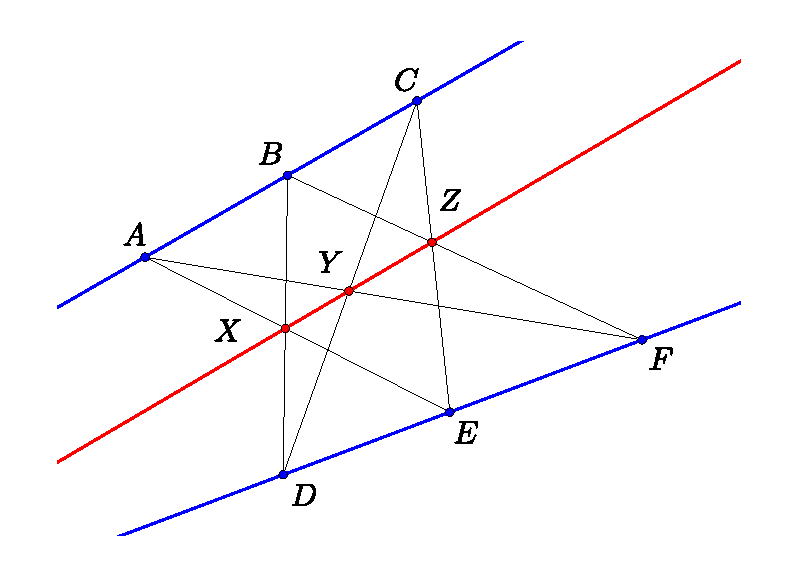
\includegraphics[width=4cm\textwidth]{imageName}
    {\scriptsize \it Lore/sensual description \\}
  \vrule width \textwidth height 1pt \\[-3pt] 
	\\\hspace\\
        {\scriptsize Mechanics/effects description  \\[5pt] \\} % <------Give a line break here
 \vfill   };

\end{tikzpicture}

&

% Wizzard Mana level 1
%
\begin{tikzpicture}
\draw[rounded corners=0.2cm] (0,0) rectangle (\cardwidth,\cardheight);
\fill[blue,rounded corners=0.1cm] (\strippadding,\strippadding) rectangle (\strippadding+\stripwidth,\cardheight-\strippadding) node[rotate=90,above left,white,font=\large] {\bf Mana \rotatebox[origin=c]{-90}{1}};
\node[text width=(\cardwidth-\strippadding-\stripwidth-2*\textpadding-0.3)*1cm,below right] at (\strippadding+\stripwidth+\textpadding,\cardheight-\textpadding) {
    {\Large Mana Crystal }\ \\\hspace\\
		%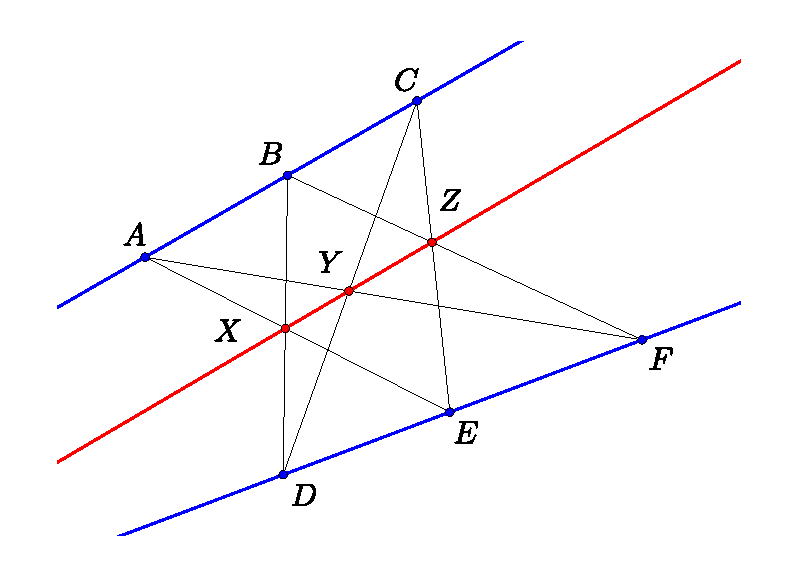
\includegraphics[width=4cm\textwidth]{imageName}
    {\scriptsize \it Crystalline structures that captured cosmic essence as they grew. \\}
  \vrule width \textwidth height 1pt \\[-3pt] 
	\\\hspace\\
        {\scriptsize Cast a spell of level 1 \\\*\\ Discard after use \\[5pt] \\} % <------Give a line break here
 \vfill   };

\end{tikzpicture}

&

% Wizzard Mana level 2
%
\begin{tikzpicture}
\draw[rounded corners=0.2cm] (0,0) rectangle (\cardwidth,\cardheight);
\fill[blue,rounded corners=0.1cm] (\strippadding,\strippadding) rectangle (\strippadding+\stripwidth,\cardheight-\strippadding) node[rotate=90,above left,white,font=\large] {\bf Mana \rotatebox[origin=c]{-90}{2}};
\node[text width=(\cardwidth-\strippadding-\stripwidth-2*\textpadding-0.3)*1cm,below right] at (\strippadding+\stripwidth+\textpadding,\cardheight-\textpadding) {
    {\Large Mana Crystal }\ \\\hspace\\
		%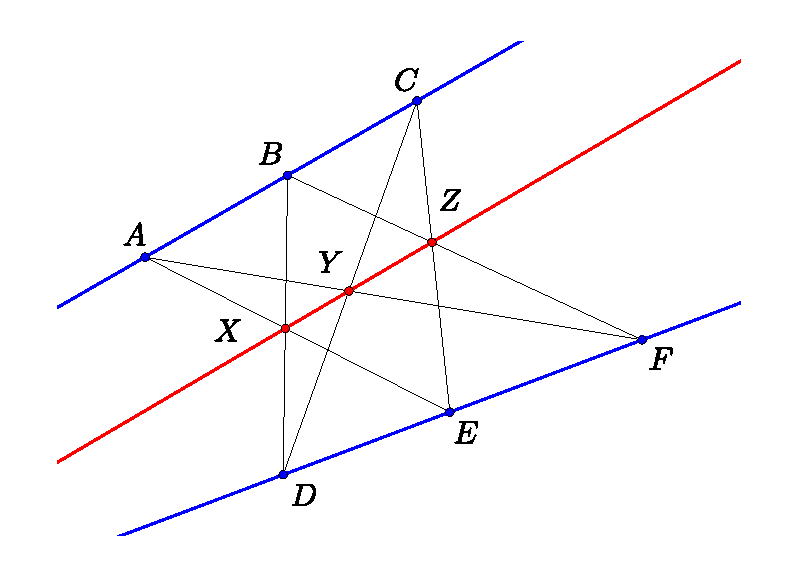
\includegraphics[width=4cm\textwidth]{imageName}
    {\scriptsize \it Crystalline structures that captured cosmic essence as they grew. \\}
  \vrule width \textwidth height 1pt \\[-3pt] 
	\\\hspace\\
        {\scriptsize Cast a spell of level 2 or lower \\\*\\ Discard after use \\[5pt] \\} % <------Give a line break here
 \vfill   };

\end{tikzpicture}

& \\

% Wizzard Mana level 3
%
\begin{tikzpicture}
\draw[rounded corners=0.2cm] (0,0) rectangle (\cardwidth,\cardheight);
\fill[blue,rounded corners=0.1cm] (\strippadding,\strippadding) rectangle (\strippadding+\stripwidth,\cardheight-\strippadding) node[rotate=90,above left,white,font=\large] {\bf Mana \rotatebox[origin=c]{-90}{3}};
\node[text width=(\cardwidth-\strippadding-\stripwidth-2*\textpadding-0.3)*1cm,below right] at (\strippadding+\stripwidth+\textpadding,\cardheight-\textpadding) {
    {\Large Mana Crystal }\ \\\hspace\\
		%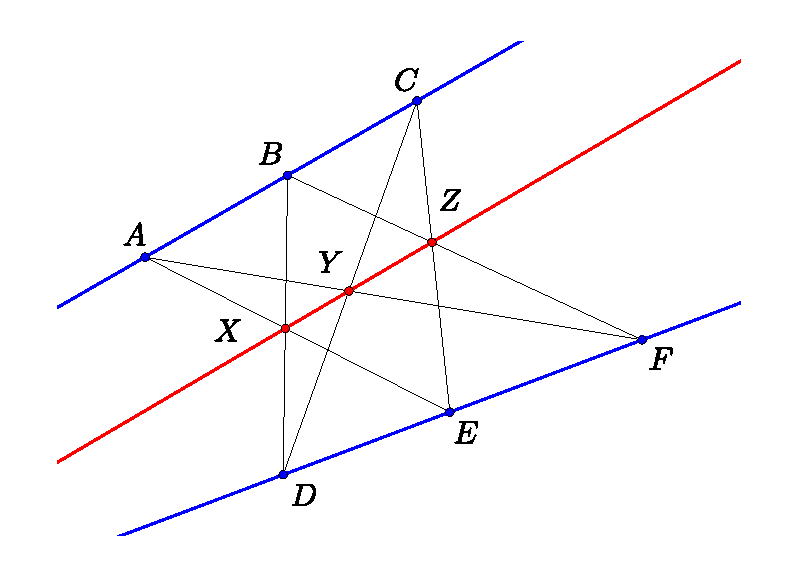
\includegraphics[width=4cm\textwidth]{imageName}
    {\scriptsize \it Crystalline structures that captured cosmic essence as they grew. \\}
  \vrule width \textwidth height 1pt \\[-3pt] 
	\\\hspace\\
        {\scriptsize Cast a spell of level 3 or lower \\\*\\ Discard after use \\[5pt] \\} % <------Give a line break here
 \vfill   };

\end{tikzpicture}

&

% Wizzard Mana level 4
%
\begin{tikzpicture}
\draw[rounded corners=0.2cm] (0,0) rectangle (\cardwidth,\cardheight);
\fill[blue,rounded corners=0.1cm] (\strippadding,\strippadding) rectangle (\strippadding+\stripwidth,\cardheight-\strippadding) node[rotate=90,above left,white,font=\large] {\bf Mana \rotatebox[origin=c]{-90}{4}};
\node[text width=(\cardwidth-\strippadding-\stripwidth-2*\textpadding-0.3)*1cm,below right] at (\strippadding+\stripwidth+\textpadding,\cardheight-\textpadding) {
    {\Large Mana Crystal }\ \\\hspace\\
		%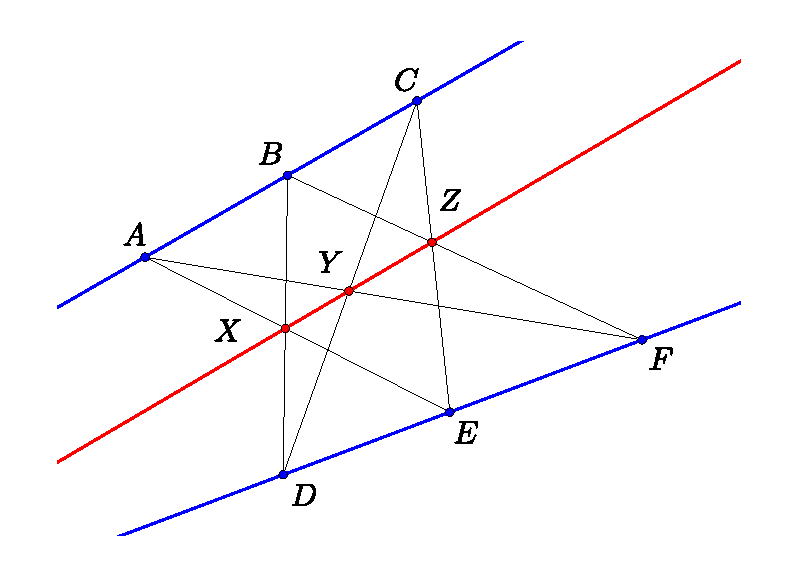
\includegraphics[width=4cm\textwidth]{imageName}
    {\scriptsize \it Crystalline structures that captured cosmic essence as they grew. \\}
  \vrule width \textwidth height 1pt \\[-3pt] 
	\\\hspace\\
        {\scriptsize Cast a spell of level 4 or lower \\\*\\ Discard after use \\[5pt] \\} % <------Give a line break here
 \vfill   };

\end{tikzpicture}

&

% Wizzard Mana level 5
%
\begin{tikzpicture}
\draw[rounded corners=0.2cm] (0,0) rectangle (\cardwidth,\cardheight);
\fill[blue,rounded corners=0.1cm] (\strippadding,\strippadding) rectangle (\strippadding+\stripwidth,\cardheight-\strippadding) node[rotate=90,above left,white,font=\large] {\bf Mana \rotatebox[origin=c]{-90}{5}};
\node[text width=(\cardwidth-\strippadding-\stripwidth-2*\textpadding-0.3)*1cm,below right] at (\strippadding+\stripwidth+\textpadding,\cardheight-\textpadding) {
    {\Large Mana Crystal }\ \\\hspace\\
		%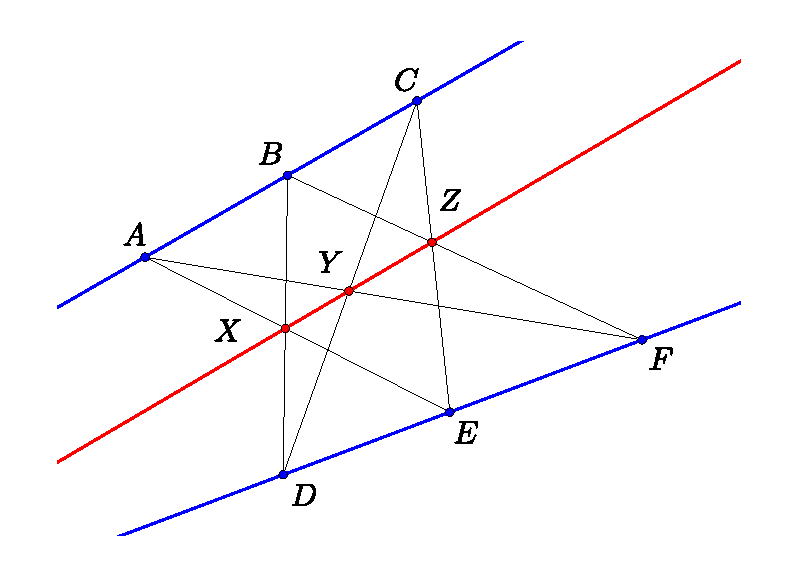
\includegraphics[width=4cm\textwidth]{imageName}
    {\scriptsize \it Crystalline structures that captured cosmic essence as they grew. \\}
  \vrule width \textwidth height 1pt \\[-3pt] 
	\\\hspace\\
        {\scriptsize Cast a spell of level 5 or lower \\\*\\ Discard after use \\[5pt] \\} % <------Give a line break here
 \vfill   };

\end{tikzpicture}

&\\

% Wizzard Mana level 6
%
\begin{tikzpicture}
\draw[rounded corners=0.2cm] (0,0) rectangle (\cardwidth,\cardheight);
\fill[blue,rounded corners=0.1cm] (\strippadding,\strippadding) rectangle (\strippadding+\stripwidth,\cardheight-\strippadding) node[rotate=90,above left,white,font=\large] {\bf Mana \rotatebox[origin=c]{-90}{6}};
\node[text width=(\cardwidth-\strippadding-\stripwidth-2*\textpadding-0.3)*1cm,below right] at (\strippadding+\stripwidth+\textpadding,\cardheight-\textpadding) {
    {\Large Mana Crystal }\ \\\hspace\\
		%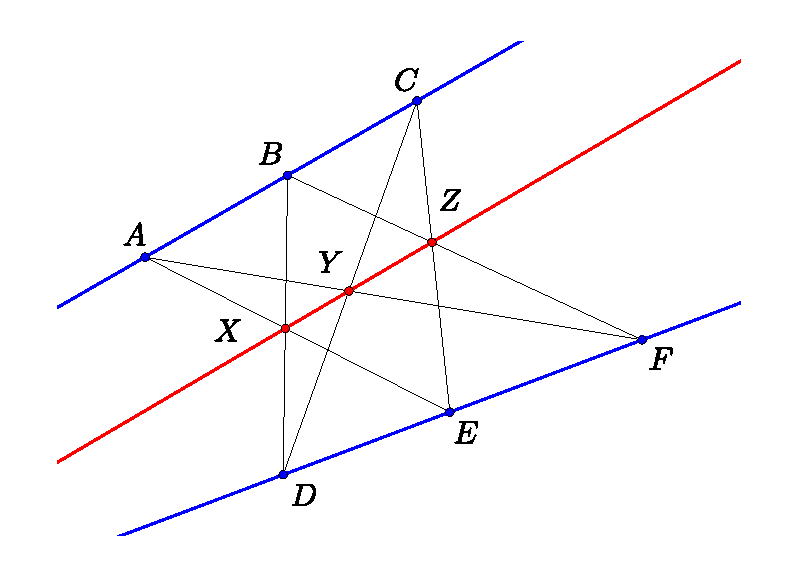
\includegraphics[width=4cm\textwidth]{imageName}
    {\scriptsize \it Crystalline structures that captured cosmic essence as they grew. \\}
  \vrule width \textwidth height 1pt \\[-3pt] 
	\\\hspace\\
        {\scriptsize Cast a spell of level 6 or lower \\\*\\ Discard after use \\[5pt] \\} % <------Give a line break here
 \vfill   };

\end{tikzpicture}

&

% Wizzard Mana level 7
%
\begin{tikzpicture}
\draw[rounded corners=0.2cm] (0,0) rectangle (\cardwidth,\cardheight);
\fill[blue,rounded corners=0.1cm] (\strippadding,\strippadding) rectangle (\strippadding+\stripwidth,\cardheight-\strippadding) node[rotate=90,above left,white,font=\large] {\bf Mana \rotatebox[origin=c]{-90}{7}};
\node[text width=(\cardwidth-\strippadding-\stripwidth-2*\textpadding-0.3)*1cm,below right] at (\strippadding+\stripwidth+\textpadding,\cardheight-\textpadding) {
    {\Large Mana Crystal }\ \\\hspace\\
		%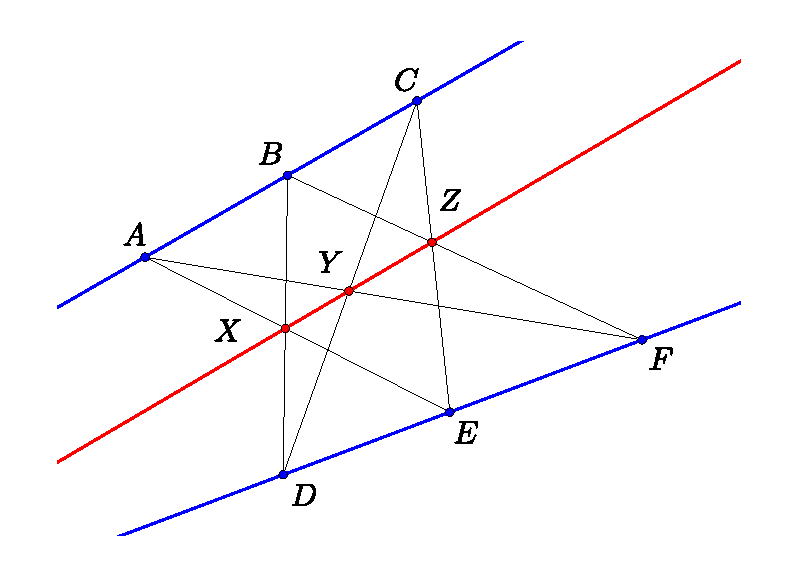
\includegraphics[width=4cm\textwidth]{imageName}
    {\scriptsize \it Crystalline structures that captured cosmic essence as they grew. \\}
  \vrule width \textwidth height 1pt \\[-3pt] 
	\\\hspace\\
        {\scriptsize Cast a spell of level 7 or lower \\\*\\ Discard after use \\[5pt] \\} % <------Give a line break here
 \vfill   };

\end{tikzpicture}

&

% Wizzard Mana level 8
%
\begin{tikzpicture}
\draw[rounded corners=0.2cm] (0,0) rectangle (\cardwidth,\cardheight);
\fill[blue,rounded corners=0.1cm] (\strippadding,\strippadding) rectangle (\strippadding+\stripwidth,\cardheight-\strippadding) node[rotate=90,above left,white,font=\large] {\bf Mana \rotatebox[origin=c]{-90}{8}};
\node[text width=(\cardwidth-\strippadding-\stripwidth-2*\textpadding-0.3)*1cm,below right] at (\strippadding+\stripwidth+\textpadding,\cardheight-\textpadding) {
    {\Large Mana Crystal }\ \\\hspace\\
		%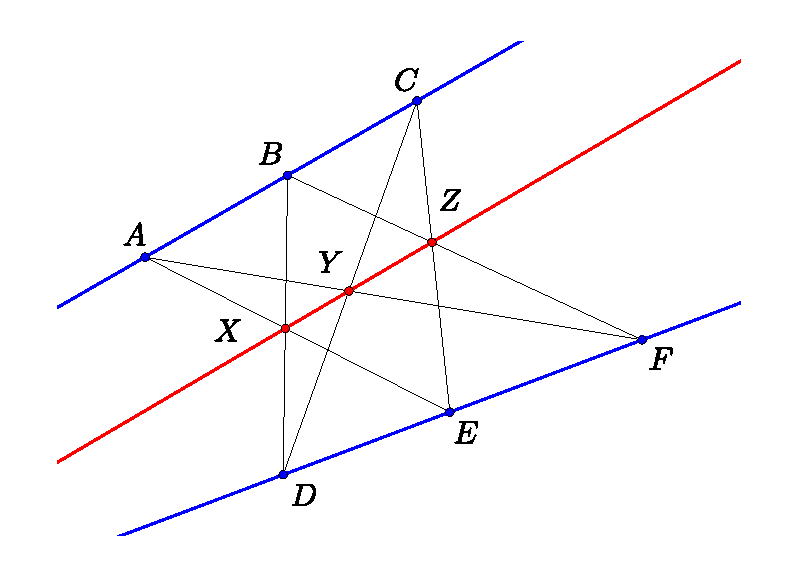
\includegraphics[width=4cm\textwidth]{imageName}
    {\scriptsize \it Crystalline structures that captured cosmic essence as they grew. \\}
  \vrule width \textwidth height 1pt \\[-3pt] 
	\\\hspace\\
        {\scriptsize Cast a spell of level 8 or lower \\\*\\ Discard after use \\[5pt] \\} % <------Give a line break here
 \vfill   };

\end{tikzpicture}

\end{tabular}



\newpage

%page 2
\begin{tabular}{ccc}

% Card layout
%
\begin{tikzpicture}
\draw[rounded corners=0.2cm] (0,0) rectangle (\cardwidth,\cardheight);
\fill[blue,rounded corners=0.1cm] (\strippadding,\strippadding) rectangle (\strippadding+\stripwidth,\cardheight-\strippadding) node[rotate=90,above left,white,font=\large] {\bf Color = (sub)class - Spell Name \rotatebox[origin=c]{-90}{1}};
\node[text width=(\cardwidth-\strippadding-\stripwidth-2*\textpadding-0.3)*1cm,below right] at (\strippadding+\stripwidth+\textpadding,\cardheight-\textpadding) {
    {\Large  }\ \\\hspace\\
		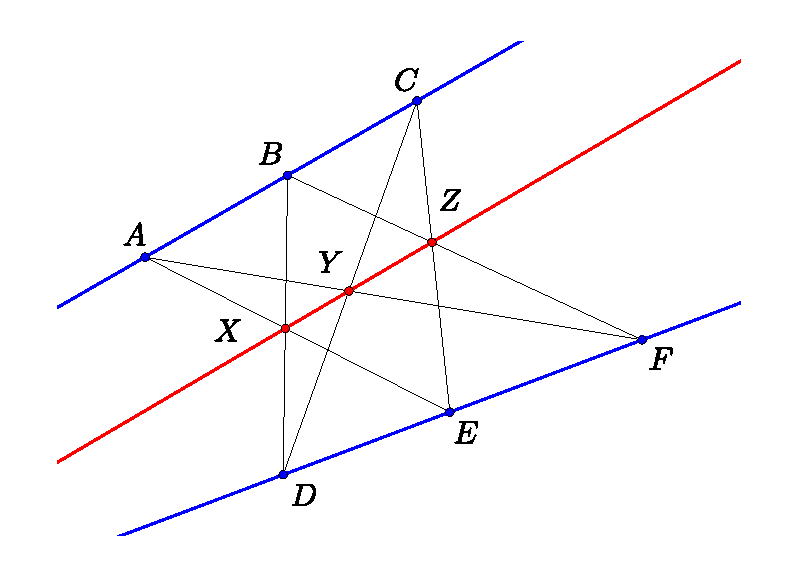
\includegraphics[width=4cm\textwidth]{imageName}
    {\scriptsize \it Lore/sensual description \\}
  \vrule width \textwidth height 1pt \\[-3pt] 
	\\\hspace\\
        {\scriptsize Mechanics/effects description  \\[5pt] \\} % <------Give a line break here
 \vfill   };

\end{tikzpicture}

&

% For program
%
\begin{tikzpicture}
\draw[rounded corners=0.2cm] (0,0) rectangle (\cardwidth,\cardheight);
\fill[@color,rounded corners=0.1cm] (\strippadding,\strippadding) rectangle (\strippadding+\stripwidth,\cardheight-\strippadding) node[rotate=90,above left,white,font=\large] {\rotatebox[origin=c]{-90}{@C} \bf @spellName \rotatebox[origin=c]{-90}{@L}};
\node[text width=(\cardwidth-\strippadding-\stripwidth-2*\textpadding-0.3)*1cm,below right] at (\strippadding+\stripwidth+\textpadding,\cardheight-\textpadding) {
    {\Large @spellName \\}
		{\scriptsize \it if@saveThrow\\\*\\}
		{\scriptsize \bf Target:\,\,}{\scriptsize @targetArea\\}
		{\scriptsize \bf Range:\,\,}{\scriptsize @range\\}		
		{\scriptsize \bf Roll:\,\,}{\scriptsize @damage\,\,}{\scriptsize \it if@damageType}
  \vrule width \textwidth height 1pt \\[-3pt] 
	\\\hspace\\
	{\scriptsize \it @detail \\}
        {\scriptsize if@higherLv} % <------Give a line break here
 \vfill   
{\scriptsize if@components (@pageNumber)} };

\end{tikzpicture}

&

% Wizzard Mana level 2
%
\begin{tikzpicture}
\draw[rounded corners=0.2cm] (0,0) rectangle (\cardwidth,\cardheight);
\fill[darkgreen,rounded corners=0.1cm] (\strippadding,\strippadding) rectangle (\strippadding+\stripwidth,\cardheight-\strippadding) node[rotate=90,above left,white,font=\large] {\rotatebox[origin=c]{-90}{W} \bf (Conjuration) Acid Splash \rotatebox[origin=c]{-90}{1}};
\node[text width=(\cardwidth-\strippadding-\stripwidth-2*\textpadding-0.3)*1cm,below right] at (\strippadding+\stripwidth+\textpadding,\cardheight-\textpadding) {
    {\Large Acid Splash\\}
		{\scriptsize \it Saving Throw: Dex\\\*\\}
		%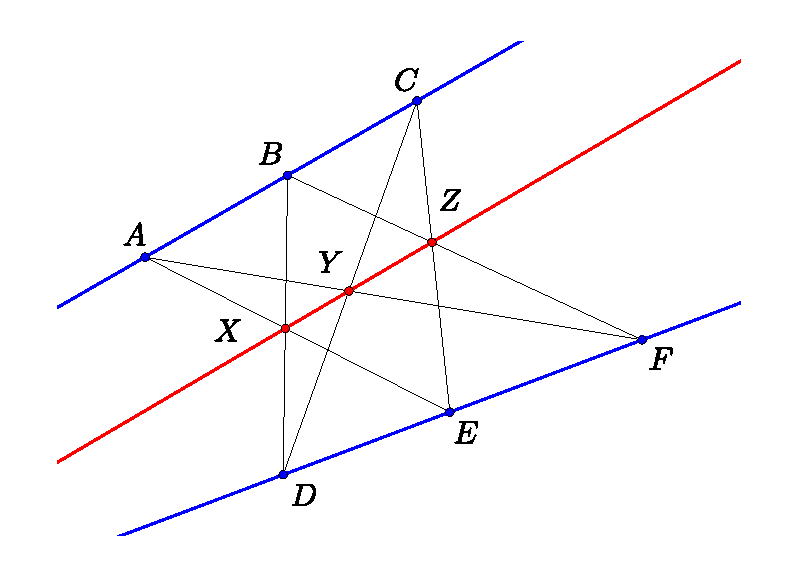
\includegraphics[width=4cm\textwidth]{imageName}
		{\scriptsize \bf Target:\,\,}{\scriptsize 1 or 2 adjacent targets\\}
		{\scriptsize \bf Range:\,\,}{\scriptsize 60 ft.\\}		
		{\scriptsize \bf Roll:\,\,}{\scriptsize DAM: 1d6\,\,}{\scriptsize \it (Acid)}
  \vrule width \textwidth height 1pt \\[-3pt] 
	\\\hspace\\
	{\scriptsize \it DAM: Add extra 1d6 at 5th level, 11th level, and 17th level. }
        {\scriptsize Cast a spell of level 2 or lower \\\*\\ Discard after use \\[5pt] \\} % <------Give a line break here
 \vfill   };

\end{tikzpicture}

& \\

% Wizzard Mana level 3
%
\begin{tikzpicture}
\draw[rounded corners=0.2cm] (0,0) rectangle (\cardwidth,\cardheight);
\fill[blue,rounded corners=0.1cm] (\strippadding,\strippadding) rectangle (\strippadding+\stripwidth,\cardheight-\strippadding) node[rotate=90,above left,white,font=\large] {\bf Mana \rotatebox[origin=c]{-90}{3}};
\node[text width=(\cardwidth-\strippadding-\stripwidth-2*\textpadding-0.3)*1cm,below right] at (\strippadding+\stripwidth+\textpadding,\cardheight-\textpadding) {
    {\Large Mana Crystal }\ \\\hspace\\
		%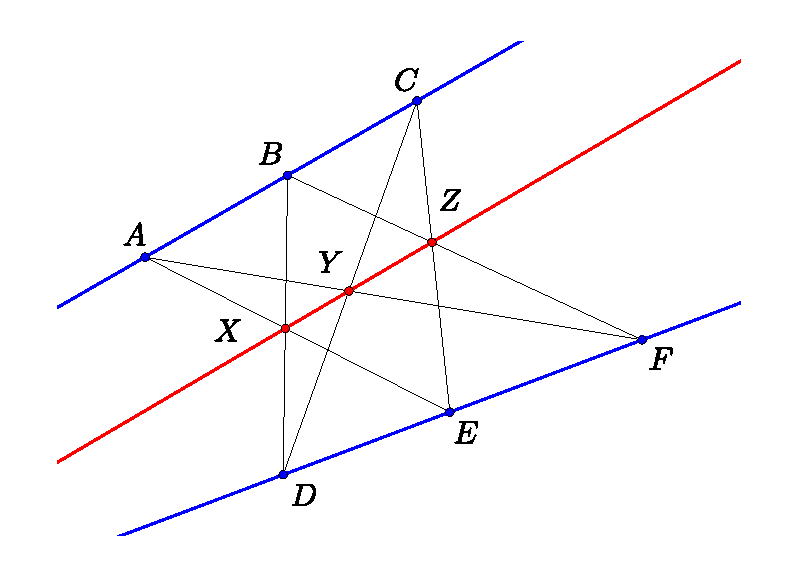
\includegraphics[width=4cm\textwidth]{imageName}
    {\scriptsize \it Crystalline structures that captured cosmic essence as they grew. \\}
  \vrule width \textwidth height 1pt \\[-3pt] 
	\\\hspace\\
        {\scriptsize Cast a spell of level 3 or lower \\\*\\ Discard after use \\[5pt] \\} % <------Give a line break here
 \vfill   };

\end{tikzpicture}

&

% Wizzard Mana level 4
%
\begin{tikzpicture}
\draw[rounded corners=0.2cm] (0,0) rectangle (\cardwidth,\cardheight);
\fill[blue,rounded corners=0.1cm] (\strippadding,\strippadding) rectangle (\strippadding+\stripwidth,\cardheight-\strippadding) node[rotate=90,above left,white,font=\large] {\bf Mana \rotatebox[origin=c]{-90}{4}};
\node[text width=(\cardwidth-\strippadding-\stripwidth-2*\textpadding-0.3)*1cm,below right] at (\strippadding+\stripwidth+\textpadding,\cardheight-\textpadding) {
    {\Large Mana Crystal }\ \\\hspace\\
		%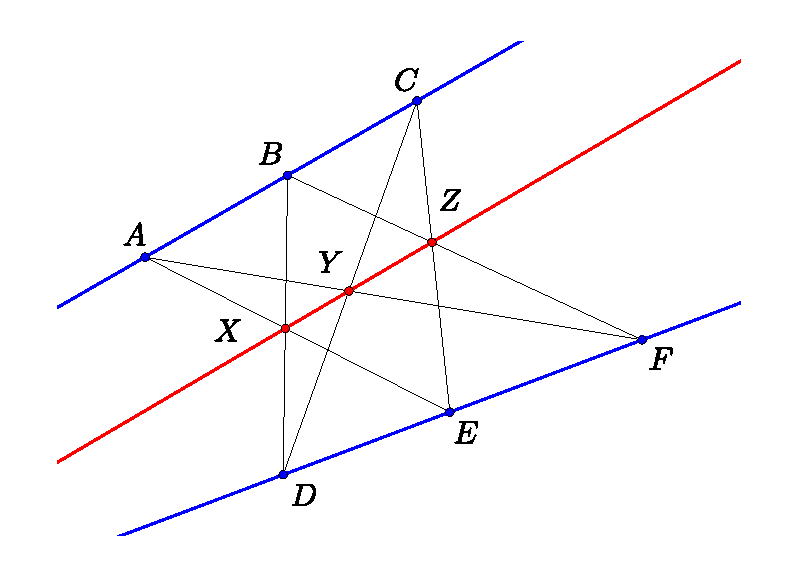
\includegraphics[width=4cm\textwidth]{imageName}
    {\scriptsize \it Crystalline structures that captured cosmic essence as they grew. \\}
  \vrule width \textwidth height 1pt \\[-3pt] 
	\\\hspace\\
        {\scriptsize Cast a spell of level 4 or lower \\\*\\ Discard after use \\[5pt] \\} % <------Give a line break here
 \vfill   };

\end{tikzpicture}

&

% Wizzard Mana level 5
%
\begin{tikzpicture}
\draw[rounded corners=0.2cm] (0,0) rectangle (\cardwidth,\cardheight);
\fill[blue,rounded corners=0.1cm] (\strippadding,\strippadding) rectangle (\strippadding+\stripwidth,\cardheight-\strippadding) node[rotate=90,above left,white,font=\large] {\bf Mana \rotatebox[origin=c]{-90}{5}};
\node[text width=(\cardwidth-\strippadding-\stripwidth-2*\textpadding-0.3)*1cm,below right] at (\strippadding+\stripwidth+\textpadding,\cardheight-\textpadding) {
    {\Large Mana Crystal }\ \\\hspace\\
		%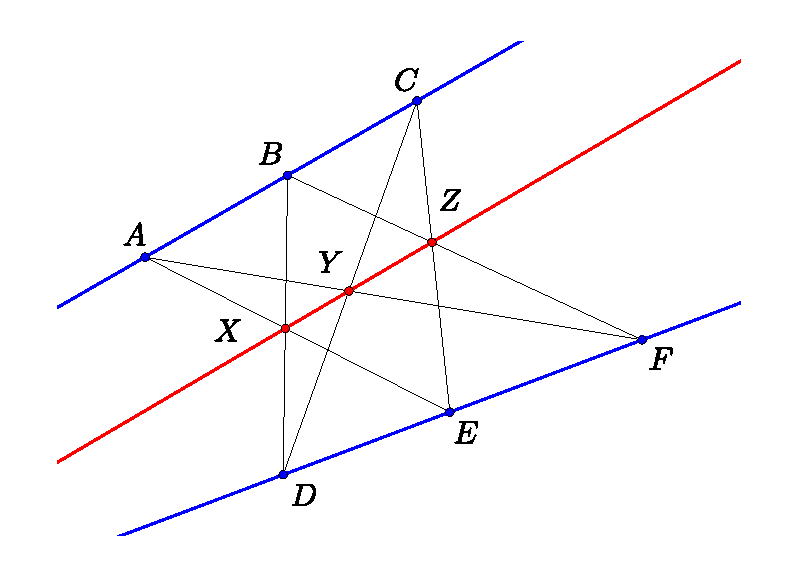
\includegraphics[width=4cm\textwidth]{imageName}
    {\scriptsize \it Crystalline structures that captured cosmic essence as they grew. \\}
  \vrule width \textwidth height 1pt \\[-3pt] 
	\\\hspace\\
        {\scriptsize Cast a spell of level 5 or lower \\\*\\ Discard after use \\[5pt] \\} % <------Give a line break here
 \vfill   };

\end{tikzpicture}

&\\

% Wizzard Mana level 6
%
\begin{tikzpicture}
\draw[rounded corners=0.2cm] (0,0) rectangle (\cardwidth,\cardheight);
\fill[blue,rounded corners=0.1cm] (\strippadding,\strippadding) rectangle (\strippadding+\stripwidth,\cardheight-\strippadding) node[rotate=90,above left,white,font=\large] {\bf Mana \rotatebox[origin=c]{-90}{6}};
\node[text width=(\cardwidth-\strippadding-\stripwidth-2*\textpadding-0.3)*1cm,below right] at (\strippadding+\stripwidth+\textpadding,\cardheight-\textpadding) {
    {\Large Mana Crystal }\ \\\hspace\\
		%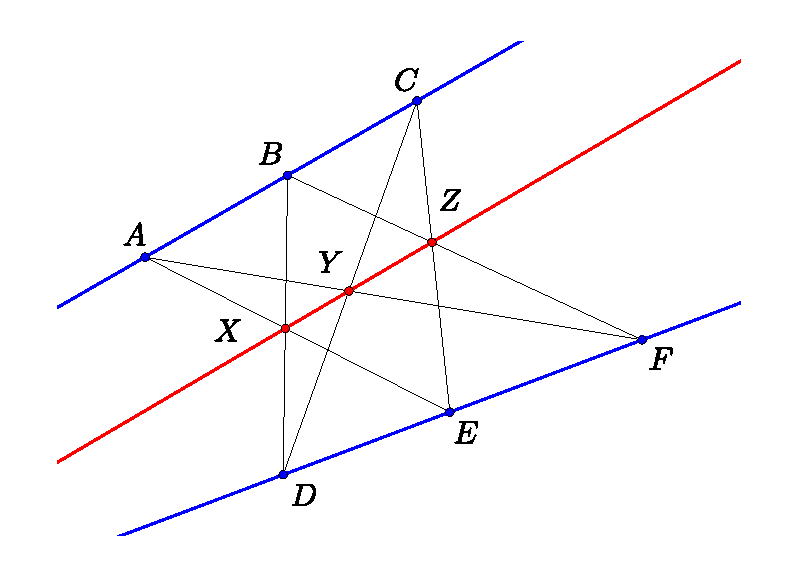
\includegraphics[width=4cm\textwidth]{imageName}
    {\scriptsize \it Crystalline structures that captured cosmic essence as they grew. \\}
  \vrule width \textwidth height 1pt \\[-3pt] 
	\\\hspace\\
        {\scriptsize Cast a spell of level 6 or lower \\\*\\ Discard after use \\[5pt] \\} % <------Give a line break here
 \vfill   };

\end{tikzpicture}

&

% Wizzard Mana level 7
%
\begin{tikzpicture}
\draw[rounded corners=0.2cm] (0,0) rectangle (\cardwidth,\cardheight);
\fill[blue,rounded corners=0.1cm] (\strippadding,\strippadding) rectangle (\strippadding+\stripwidth,\cardheight-\strippadding) node[rotate=90,above left,white,font=\large] {\bf Mana \rotatebox[origin=c]{-90}{7}};
\node[text width=(\cardwidth-\strippadding-\stripwidth-2*\textpadding-0.3)*1cm,below right] at (\strippadding+\stripwidth+\textpadding,\cardheight-\textpadding) {
    {\Large Mana Crystal }\ \\\hspace\\
		%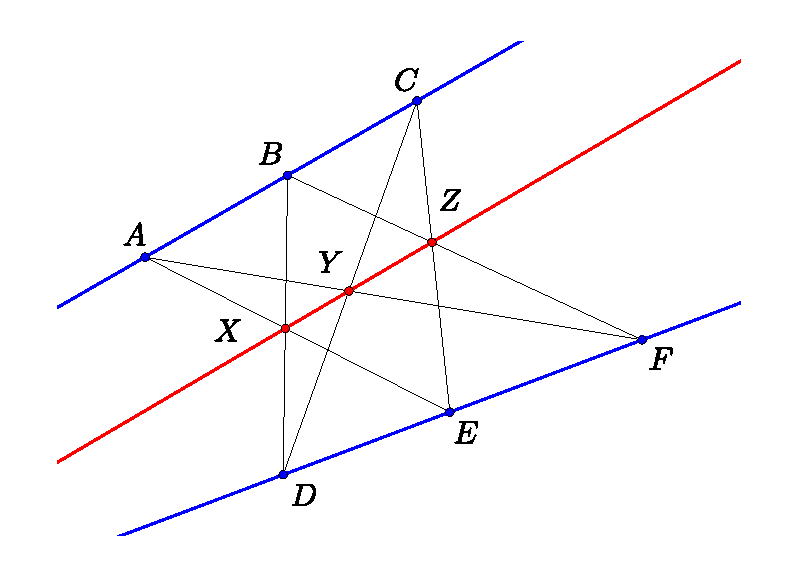
\includegraphics[width=4cm\textwidth]{imageName}
    {\scriptsize \it Crystalline structures that captured cosmic essence as they grew. \\}
  \vrule width \textwidth height 1pt \\[-3pt] 
	\\\hspace\\
        {\scriptsize Cast a spell of level 7 or lower \\\*\\ Discard after use \\[5pt] \\} % <------Give a line break here
 \vfill   };

\end{tikzpicture}

&

% Wizzard Mana level 8
%
\begin{tikzpicture}
\draw[rounded corners=0.2cm] (0,0) rectangle (\cardwidth,\cardheight);
\fill[blue,rounded corners=0.1cm] (\strippadding,\strippadding) rectangle (\strippadding+\stripwidth,\cardheight-\strippadding) node[rotate=90,above left,white,font=\large] {\bf Mana \rotatebox[origin=c]{-90}{8}};
\node[text width=(\cardwidth-\strippadding-\stripwidth-2*\textpadding-0.3)*1cm,below right] at (\strippadding+\stripwidth+\textpadding,\cardheight-\textpadding) {
    {\Large Mana Crystal }\ \\\hspace\\
		%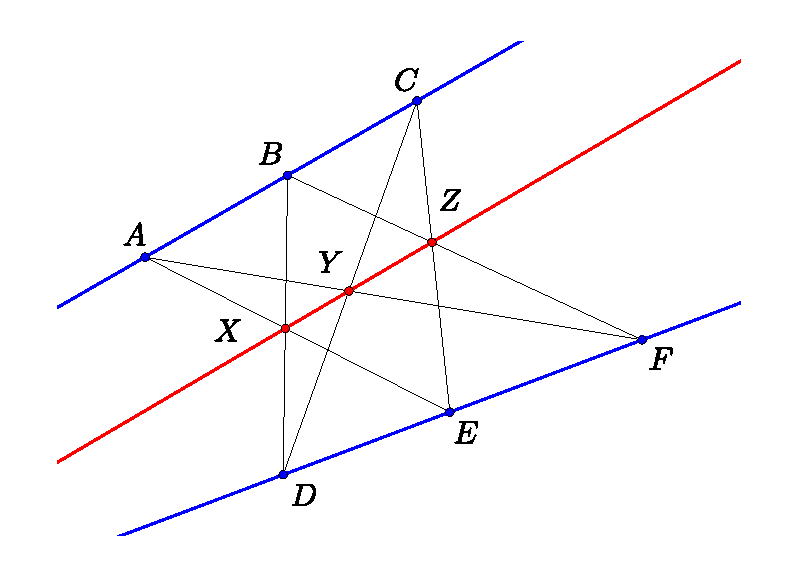
\includegraphics[width=4cm\textwidth]{imageName}
    {\scriptsize \it Crystalline structures that captured cosmic essence as they grew. \\}
  \vrule width \textwidth height 1pt \\[-3pt] 
	\\\hspace\\
        {\scriptsize Cast a spell of level 8 or lower \\\*\\ Discard after use \\[5pt] \\} % <------Give a line break here
 \vfill   };

\end{tikzpicture}

\end{tabular}





\end{document}